% Mid-term report: Choosing Which Links to Check
% Compile with:  pdflatex main.tex   (run twice so references resolve)
% Figures are in the figures/ folder next to this file.

\documentclass[11pt,a4paper]{article}

\usepackage[utf8]{inputenc}
\usepackage[T1]{fontenc}
\usepackage{lmodern}
\usepackage[margin=1in]{geometry}
\usepackage{graphicx}
\usepackage{booktabs}
\usepackage{tabularx}
\usepackage{array}
\usepackage{amsmath}
\usepackage{xcolor}
\usepackage{caption}
\usepackage{enumitem}
\usepackage[hidelinks]{hyperref}

\graphicspath{{figures/}}
\captionsetup{font=small,labelfont=bf}
\setlength{\parskip}{0.5em}
\setlength{\parindent}{0pt}

% Red "[verify]" marks for claims about papers you have not read closely.
% Change \showverifytrue to \showverifyfalse to hide them all.
\newif\ifshowverify
\showverifytrue
\newcommand{\verify}{\ifshowverify\textcolor{red}{\textsuperscript{[verify]}}\fi}

% ---------- Fill these in ----------
\newcommand{\reporttitle}{Active Link Acquisition on Partially Observed Graphs:\\[0.3em] A Task-Aware Query Strategy for Graph-Based Inference}
\newcommand{\studentname}{Pragunie Aditya}
\newcommand{\rollno}{2310110682}
\newcommand{\supervisor}{Dr. Suchi Kumari}
\newcommand{\supervisortitle}{Assistant Professor, Department of Computer Science and Engineering}
\newcommand{\university}{Shiv Nadar University, Delhi NCR}
\newcommand{\department}{Department of Computer Science and Engineering}
\newcommand{\reportdate}{October, 2025}
% -----------------------------------

\begin{document}

% ======================= Title page =======================
\begin{titlepage}
\centering
\vspace*{1.0cm}
{\LARGE \reporttitle \par}
\vspace{1.2cm}
{\large Mid-Term Project Report Submitted in Partial Fulfilment of the Requirements for the Degree of\par}
\vspace{0.5cm}
{\Large\bfseries Bachelor of Technology\par}
{\itshape in\par}
{\Large\bfseries Computer Science and Engineering\par}
\vspace{1.5cm}
{\itshape Submitted by}\\[0.3em]
{\bfseries \studentname}\ (Roll No.\ \rollno)\\[1.5cm]
{\itshape Under the Supervision of}\\[0.3em]
{\bfseries \supervisor}\\[0.2em]
\supervisortitle\\[0.2em]
\university
\vfill
{\bfseries \department}\\[0.3em]
{\bfseries \university}\\[0.3em]
\reportdate
\end{titlepage}

% ======================= Declaration =======================
\newpage
\section*{Declaration}
I/We declare that this written submission represents my ideas in my own words and where others'
ideas or words have been included, I have adequately cited and referenced the original sources. I
also declare that I have adhered to all principles of academic honesty and integrity and have not
misrepresented or fabricated or falsified any idea/data/fact/source in my submission. I understand
that any violation of the above will be cause for disciplinary action by the University and can also
evoke penal action from the sources which have thus not been properly cited or from whom proper
permission has not been taken when needed.

\vspace{1.5cm}
\noindent\textbf{Name of the Student:} \studentname\\[0.5cm]
\noindent\textbf{Signature and Date:}
\raisebox{-0.8cm}{\includegraphics[height=2cm]{figures/signature_pragunie.jpg}}
\hfill \textbf{14-10-2025}

\vspace{1.5cm}
\noindent\textbf{Faculty Advisor:} \supervisor\\[1.5cm]
\noindent\textbf{Signature:} \rule{5cm}{0.4pt} \hfill \textbf{14-10-2025}
\newpage

% ======================= Abstract =======================
\begin{abstract}
Graph-structured data arising from social, biological, and information networks is frequently
only partially observed, as verifying the existence of a link between two entities may require
expert knowledge, experimental effort, or restricted data access. Given a fixed budget of such
verification queries, this project investigates which candidate links should be prioritised so
that a designated set of target nodes can be classified as accurately as possible. We introduce
a task-aware query scoring framework in which each candidate link is evaluated by its expected
contribution to the classifier's confidence on the target nodes, weighted by the estimated
probability that the link exists. The classifier employed is label propagation, whose closed-form
solution permits exact evaluation of every candidate without model retraining. On synthetic
community-structured graphs generated under the Contextual Stochastic Block Model, we find that
strategies that maximise the number of true links discovered do not maximise classification
accuracy on the targets. In contrast, the proposed task-aware strategy closes 45--53\,\% of the
accuracy gap between a partially observed and a fully observed network within 200 queries,
compared with at most 13\,\% for standard link-prediction and uncertainty-based heuristics.
These findings replicate on held-out random seeds and remain stable under three distinct
link-hiding schemes. The project further examines the incremental benefit of adaptive
(sequential) query selection and characterises the role of target reachability as the primary
mechanism underlying accuracy improvement. Limitations of the current study and directions for
future work are discussed.
\end{abstract}

% ======================= 1 Introduction =======================
\section{Introduction: Background and Motivation}

Relational data from domains such as social networks, citation networks, biological interaction
networks, and knowledge graphs are naturally represented as graphs, where nodes correspond to
entities and edges encode pairwise relationships. A fundamental operation on such graphs is
node classification: assigning each node to one of several discrete categories based on its
position in the network and, optionally, its attributes. In practice, however, the observed
graph is almost never complete. Confirming whether an edge between two entities exists may
require expert annotation, experimental assay, or a paid data access request---each carrying
a non-trivial cost. Consequently, the practitioner faces a budget-constrained setting in which
only a limited number of edge verification queries can be issued.

The problem of deciding \emph{which} edges to verify has received attention under the framing
of active link prediction, where the goal is to recover as many true links as possible within
the allotted budget. However, recovering more true links does not necessarily translate into
better performance on the downstream inference task. An edge that connects two already-labelled
nodes, or two nodes that are structurally isolated from any labelled node, contributes no
information to a propagation-based classifier regardless of whether it is observed. This
motivates a shift from link-centric to \emph{task-centric} query selection: choosing edges
not because they are likely to exist, but because discovering them is expected to improve
the classifier's predictions on a designated set of target nodes.

This project develops and evaluates a task-aware active link acquisition framework. Given a
partially observed graph, a set of labelled nodes, a set of target nodes whose labels are to
be inferred, and a fixed query budget, our method scores each candidate edge by its expected
contribution to classification accuracy on the target nodes. Queries are issued either
adaptively (one at a time, with the scoring updated after each answer) or statically (all
queries planned before the first answer is received). The classifier used throughout is label
propagation, whose closed-form solution enables exact, retraining-free evaluation of every
candidate edge.

\subsection{Research Questions}

\begin{enumerate}[leftmargin=3.4em,labelwidth=3em,align=left]
\item[\textbf{RQ1}] Does recovering more true edges lead to higher classification accuracy on
the target nodes, or do link-finding rate and task accuracy decouple?
\item[\textbf{RQ2}] Does task-aware query selection outperform link-prediction heuristics and
generic uncertainty sampling when the evaluation criterion is target accuracy?
\item[\textbf{RQ3}] Does adaptive (sequential) query planning yield additional accuracy gains
over static planning, and at what point in the budget does this benefit emerge?
\item[\textbf{RQ4}] Are the findings robust to different random seeds, different link-hiding
schemes, and restriction of the query space to the neighbourhood of the target nodes?
\end{enumerate}

\subsection{Objectives}

\begin{enumerate}[leftmargin=2em]
\item To construct a controlled experimental benchmark for evaluating edge-query strategies
on partially observed graphs with a designated target set and a fixed verification budget.
\item To demonstrate and quantify the divergence between link-finding performance and
downstream classification accuracy on the target nodes.
\item To design and implement a task-aware value scoring strategy that ranks candidate edges
by expected improvement in classifier confidence on the target nodes, and to compare it against
structural link-prediction heuristics and generic uncertainty sampling under both static and
adaptive planning modes.
\item To assess the robustness of the proposed strategy through replication on held-out random
seeds, evaluation under three distinct link-hiding mechanisms, and restriction of the query
space to the frontier of the target nodes' reachable subgraph.
\end{enumerate}

% ======================= 2 Literature review =======================
\section{Literature Review}

The problem of active link acquisition for downstream graph inference draws on several lines
of prior work. We organise the review from foundational link prediction methods, through
classical machine learning and neural approaches, to active and task-aware learning frameworks.

\subsection{Classical Link Prediction}

Link prediction---estimating whether a missing edge exists between two nodes---has been
studied extensively using structural similarity indices derived from the graph topology.
Adamic and Adar~\cite{adamic} proposed a score based on the inverse-log-frequency of common
neighbours, motivated by the intuition that rare common contacts carry more information than
popular ones. Jaccard similarity and the Common Neighbours count are similar
neighbourhood-overlap heuristics. Katz centrality generalises these by summing weighted
paths of all lengths between a pair of nodes. Resource Allocation and the preferential
attachment score (product of degrees) likewise exploit structural properties. These
methods are fast, parameter-free, and interpretable, but they optimise only for edge
existence and carry no information about how a predicted edge would affect a downstream
inference task.

\subsection{Classical Machine Learning Approaches}

Beyond purely structural measures, matrix factorisation methods such as SVD-based latent
factor models and Non-negative Matrix Factorisation learn low-dimensional node embeddings
from the adjacency matrix and predict missing entries from their inner product. Logistic
regression and support vector machines trained on hand-crafted node-pair features (degree,
common neighbours, shortest path, Katz score) represent the supervised link prediction
paradigm~\cite{settles}. These approaches improved over structural heuristics, particularly
on sparse graphs, but they are generally batch methods: a model is trained once on a fixed
observation and then applied, with no mechanism for adaptively choosing which edges to observe.

\subsection{Neural Network and Graph Neural Network Approaches}

Graph Autoencoders and Variational Graph Autoencoders~\cite{kipf} introduced end-to-end
learning of node embeddings from both graph structure and node features for link prediction.
The encoder is a Graph Convolutional Network~\cite{kipf} that propagates feature information
over the adjacency matrix; the decoder predicts edge existence from the inner product of
latent representations. Subsequent work replaced the GCN encoder with more expressive
architectures including GraphSAGE, GAT, and SEAL (Weisfeiler-Lehman Subtree-based link
prediction), achieving strong results on standard benchmarks. These methods generalise well
across graphs but remain transductive in the sense that they require the full observed graph
at training time, and they do not address the question of which edges to observe next.

\subsection{Active Link Prediction}

The first work to treat the observation process itself as a decision problem is ALPINE by
Chen, Kang, Lijffijt, and De Bie~\cite{alpine}, which selects edges to query using a
network-embedding model of link probability and a closed-form V-optimality criterion\verify.
Its simpler selection rules---querying pairs with the highest degree or highest PageRank
score---form two of the baselines used in this project. The key difference is the objective:
ALPINE optimises for link prediction quality (recovering the true adjacency), whereas the
present work optimises for node classification accuracy on a designated target set.
ActiveLink~\cite{activelink} applies deep active learning to link prediction in knowledge
graphs\verify; it likewise targets link recovery rather than a downstream classification task.

\subsection{Active Learning on Graphs and Value-of-Information Scoring}

Active learning for node classification has been studied primarily in the label-query setting,
where the budget constrains how many node labels can be obtained. Hu et al.~\cite{gpa} learn a
transferable reinforcement-learning policy, Graph Policy Network, that selects which nodes to
label, with generalisation to unseen graphs\verify. Their setting differs from ours in that
they query labels rather than edges. Bevilacqua et al.~\cite{subgnn} learn which subgraphs to
select for subgraph GNNs; while not an active learning method, it supports the principle of
learning a selection policy over graph elements\verify.

The theoretical foundation for value-based query selection is expected error reduction, introduced
by Roy and McCallum~\cite{roy} for text classification. In this framework, the learner picks the
query whose inclusion is expected to reduce the model's generalisation error the most. Bayesian
Experimental Design~\cite{bed} provides a broader framework for optimal data collection under
uncertainty. Li et al.~\cite{li} survey deep active learning and organise query strategies into
uncertainty-based, representative, influence-based, Bayesian, and hybrid families\verify;
Ren et al.~\cite{ren} and Settles~\cite{settles} provide complementary treatments of the field.
Wilder et al.~\cite{wilder} argue that data acquisition decisions should be evaluated against the
downstream decision they support---the principle motivating our task-aware objective. Foster et
al.~\cite{foster} study amortised sequential experimental design, a framework relevant to future
work on learning a policy that replaces the value scorer at scale. Cheaper in-the-loop
approximations to expected error reduction include BALD~\cite{bald,gal}, which maximises the mutual
information between model parameters and query outcomes, and influence functions~\cite{koh},
which estimate per-instance effects via first-order Taylor approximations. Sun et al.~\cite{perbal} introduce a perturbation-based value signal for graph
active learning that is closely related in spirit to the scoring function developed in this
project\verify. Our scorer also employs perturbation: it tentatively inserts a candidate edge,
recomputes the closed-form label propagation solution, and measures the resulting change in the
classifier's confidence on the target nodes.

ActiveReach~\cite{activereach} applies active learning to the problem of answering approximate
reachability queries on large graphs\verify. The concept of reachability---whether a target node
lies on a path from a labelled node---also features centrally in our analysis as the primary
mechanism through which edge queries improve classification accuracy.

\subsection{Comparison with the Closest Work}

Table~\ref{tab:related} summarises how the most closely related papers differ from this project.
Entries marked \verify\ are based on the abstract and introduction of the cited work; the full
papers should be consulted before these comparisons are relied upon in a final submission.

\begin{table}[htbp]
\centering
\caption{Comparison of the most closely related prior work with this project.}
\label{tab:related}
\small
\begin{tabularx}{\textwidth}{>{\raggedright\arraybackslash}p{2.6cm}>{\raggedright\arraybackslash}X>{\raggedright\arraybackslash}X>{\raggedright\arraybackslash}X}
\toprule
Work & Downstream Task & What is Actively Chosen & Method\\
\midrule
ALPINE~\cite{alpine} & link prediction & edges & network embedding + closed-form criterion\\
ActiveLink~\cite{activelink}\verify & link prediction in KGs & edges & deep active learning\\
GPA~\cite{gpa}\verify & node classification & node labels & RL policy transferable across graphs\\
PerbALGraph~\cite{perbal}\verify & belief representation & nodes & perturbation-based value signal\\
ActiveReach~\cite{activereach}\verify & reachability queries & query pairs & active learning framework\\
\textbf{This project} & \textbf{node classification on a target set} & \textbf{edges} & \textbf{expected confidence gain under label propagation; adaptive or static scheduling}\\
\bottomrule
\end{tabularx}
\end{table}

\subsection{Research Gap}

Across the literature surveyed, we did not identify work that (i) selects edges to observe
one at a time, (ii) scores each candidate edge by its expected contribution to node classification
accuracy on a designated target set, and (iii) evaluates this against both structural link-prediction
heuristics and generic uncertainty-based selection in a controlled benchmark with held-out seeds and
multiple link-hiding schemes. The present project addresses this specific combination. We note that
our literature review is not yet a systematic survey; the claim of novelty should be verified against
a broader search before it is asserted in a final submission.

% ======================= 3 Methodology =======================
\section{Methodology}

\subsection{System Overview}

\begin{figure}[htbp]
\centering
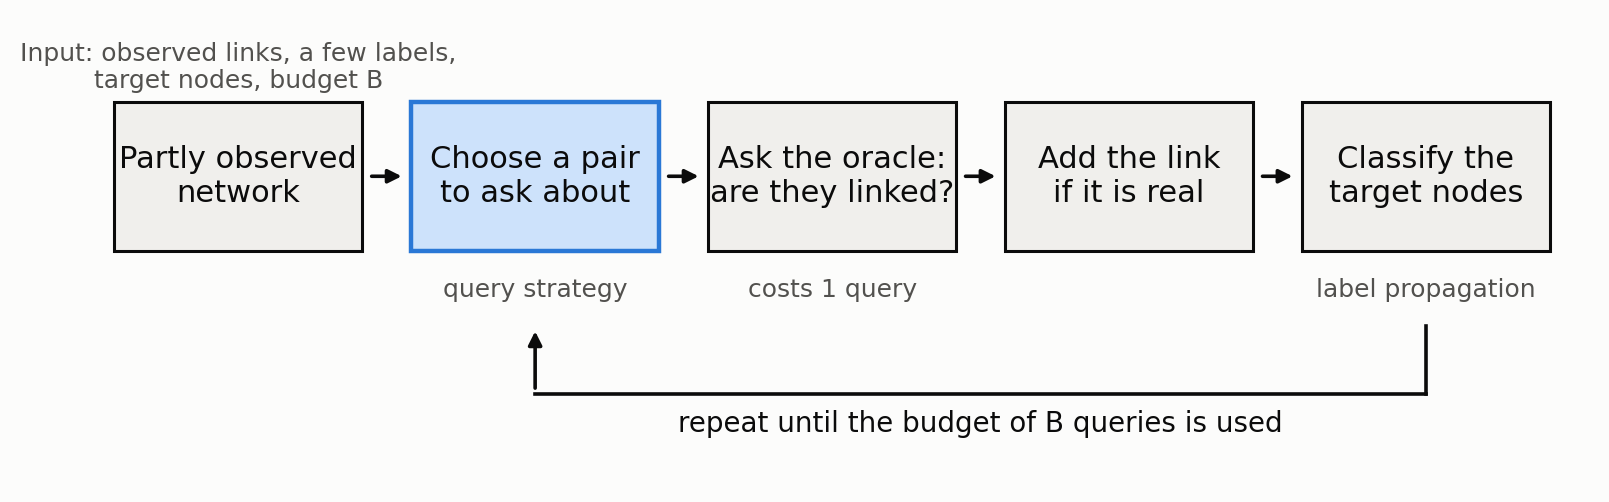
\includegraphics[width=\textwidth]{fig_pipeline.png}
\caption{End-to-end pipeline for task-aware active link acquisition. The query strategy
receives the currently observed graph, the set of labelled nodes, and the target set, and
selects the next candidate edge to verify. The oracle returns a binary answer; a confirmed
edge is incorporated into the observed graph. The classifier (label propagation) is then
re-evaluated on the target nodes. This loop repeats until the query budget is exhausted.}
\label{fig:pipeline}
\end{figure}

The framework operates as a closed-loop sequential decision process, illustrated in
Figure~\ref{fig:pipeline}. At a high level, it takes as input a partially observed graph,
a small set of labelled nodes, and a designated target set, and it outputs, for each query
step, a decision about which candidate edge to verify next. The central design principle is
that the query decision should be driven by the expected benefit for the downstream inference
task---classifying the target nodes---rather than by the likelihood of finding a true edge.

The system comprises four interacting components:

\begin{enumerate}[leftmargin=2em]
\item \textbf{The environment}: a partially observed graph generated under a community
structure model, with a fixed fraction of true edges initially revealed and the remainder
hidden from the query strategy.

\item \textbf{The oracle}: a perfect binary responder that answers each candidate-edge query
truthfully. A ``yes'' answer adds the edge to the observed graph; a ``no'' removes the pair
from the candidate pool. The oracle models the cost of link verification in the real world.

\item \textbf{The classifier}: label propagation applied to the currently observed graph. It
propagates label information from known (labelled) nodes to unlabelled nodes along observed
edges, computing, for each unlabelled node, a soft belief vector over class labels. The
classifier is the same for all query strategies; only the observed graph changes as queries
are answered.

\item \textbf{The query strategy}: the component under study. It observes the current graph
and the classifier's beliefs, scores all unqueried candidate edges, and selects one (adaptive
mode) or a ranked list (static mode) for the oracle to verify. The key distinction between
strategies is how they define ``value'' for a candidate edge.
\end{enumerate}

The framework is deliberately modular. Any of the four components can be replaced
independently. The oracle could be a noisy responder, the classifier could be a graph neural
network, and the strategy could be a learned policy rather than a hand-designed scorer. The
experiments in this project hold the oracle and classifier fixed and vary only the query
strategy, isolating the effect of task-awareness and adaptivity on downstream accuracy.

\subsection{Inputs and Outputs}

\paragraph{Inputs.}
\begin{itemize}[leftmargin=2em]
\item $G^* = (V, E^*)$: the \emph{true} graph, with $|V| = n$ nodes and $|E^*|$ edges. This
is not directly observable; only the oracle can access it.
\item $G_0 = (V, E_0)$: the \emph{initially observed} graph, where $E_0 \subseteq E^*$ is a
uniformly sampled fraction $\rho$ of the true edges ($\rho = 0.15$ in all experiments).
\item $L \subset V$: the set of \emph{labelled} nodes, with known class assignments $y_L
\in \{1, \dots, K\}^{|L|}$.
\item $T \subset V \setminus L$: the set of \emph{target} nodes, $|T| = 15$, whose class
labels are to be inferred. The labels $y_T$ are known only for evaluation; the strategy never
sees them.
\item $B$: the \emph{query budget}, the maximum number of edge queries that may be issued.
\item $\mathcal{C} \subseteq \binom{V}{2} \setminus E_0$: the set of \emph{candidate pairs},
all unobserved node pairs at the start of the process.
\end{itemize}

\paragraph{Outputs.}
\begin{itemize}[leftmargin=2em]
\item A sequence of queries $(i_1, j_1), (i_2, j_2), \dots, (i_B, j_B)$, where each pair is
selected from the candidates not yet queried.
\item For each query step $t$, an updated observed graph $G_t$ incorporating any confirmed
edges from steps $1, \dots, t$.
\item At step $B$: the predicted class labels $\hat{y}_T$ for the target nodes, derived by
applying the classifier to $G_B$. The primary evaluation metric is
$\mathrm{Acc}_T(B) = |T|^{-1} \sum_{u \in T} \mathbf{1}[\hat{y}_u = y_u]$.
\end{itemize}

\paragraph{Key intermediate quantities.}
The classifier produces, for each unlabelled node $u$, a belief vector $q_u \in \Delta^{K-1}$
over the $K$ classes. From this, three secondary quantities are tracked:
\begin{itemize}[leftmargin=2em,itemsep=0.2em]
\item \textbf{Reach}: the fraction of target nodes connected by at least one path to a
labelled node in $G_t$. Unreached nodes receive a fixed prior guess and do not benefit from
label propagation regardless of how many edges are added elsewhere.
\item \textbf{Confidence}: $\max_c q_u(c)$, the probability mass the classifier assigns to
its most likely class for node $u$.
\item \textbf{Gap closed}: $({\mathrm{Acc}_T(B) - \mathrm{Acc}_T(0)}) \;/\; (\mathrm{Acc}_T^{\mathrm{full}} - \mathrm{Acc}_T(0))$,
the fraction of the accuracy improvement between the initial partial observation and the full
graph that has been recovered by the query strategy.
\end{itemize}

\subsection{How the Approach Evolved}
The method changed in three stages, and the experiments in this report span different
stages, so we state which is which.

\textbf{Stage 1: a GCN with simple query rules.} The project started with a two-layer graph
convolutional network (hidden size 16, 100 training epochs) as the classifier, retrained from
scratch after every query. We compared random, common-neighbours (``structural'') and
uncertainty queries, and an expensive value-of-information rule that retrained the GCN once for
each candidate link. All of these runs used one fixed network, with 40\% of nodes labelled, 20\%
for validation and 40\% for testing. The first-phase results in Section~\ref{sec:prelim} come from
this stage.

\textbf{Stage 2: switching the classifier to label propagation.} Retraining a GCN for every
candidate was too slow to score more than about 15 of the roughly 4,000 candidate pairs per
query, and its estimates were noisy, so the value-of-information idea could not be tested
fairly. Label propagation has an exact closed-form answer, so the effect of any candidate link
can be computed quickly and every candidate can be scored. We therefore switched the
classifier to label propagation for the main experiments. Returning to a GCN is part of the
planned work.

\textbf{Stage 3: the task-aware setting used for the main results.} We then added a target set,
removed the validation set (the value strategy uses no labels beyond the training labels), let
the strategy estimate the link probabilities instead of being told them, generated a new
network for every seed, and evaluated on the targets. The preliminary findings in
Section~\ref{sec:prelim} and the discussion (Section~\ref{sec:discussion}) use this stage. The
attributes check and the link-weight side study used the stage-2 setup, as noted where they
appear.

\subsection{The problem in simple terms}
There is a hidden network. We can see a random 15\% of its links. A small share of the nodes
(15\% or 40\%) have known labels. We are given 15 \textbf{target nodes} whose labels are
unknown. We can ask up to $B$ queries; the oracle replies whether a pair is linked, and a
real link is added to what we can see. After the queries, a classifier predicts the targets'
labels. We want as many of those predictions as possible to be right. Figure~\ref{fig:pipeline}
shows the loop.

Two clarifications. First, the word ``query'' in this report means one question to the oracle
about one pair of nodes. The user's request (``classify these nodes'') is simulated as a random
set of 15 target nodes; we do not parse natural-language requests. Second, a ``no'' answer is
not used as evidence; it only removes that pair from the candidates.

\subsection{Formal Problem Statement}
Let $V$ be the set of $n$ nodes and let $A^{*}$ be the true (hidden) adjacency matrix. After
$t$ queries we observe a graph with adjacency matrix $A_t$, where $A_0$ contains a random 15\%
of the true links. A set $L\subset V$ of nodes has known labels $y_L$, and $T\subset V\setminus L$
is the set of target nodes. A query names a pair $(i,j)$ that has not been asked about; the
oracle returns $A^{*}_{ij}\in\{0,1\}$, and if it is 1 the link is added: $A_{t+1}=A_t+e_{ij}$.
A strategy is a rule that picks the next pair from $A_t$, $y_L$ and $T$. A fixed classifier $f$
maps $(A_t,y_L)$ to predicted labels $\hat y_u$. The aim is to maximise the accuracy on the
targets after $B$ queries,
\begin{equation}
\mathrm{Acc}_T(B)=\frac{1}{|T|}\sum_{u\in T}\mathbf{1}\bigl[\hat y_u=y_u\bigr].
\end{equation}
The strategy and the classifier are separate: we hold $f$ fixed and study only which queries
to ask. The strategy never sees the labels of nodes outside $L$ or the true probabilities of
a link.

\subsection{Synthetic Network Generation (Contextual Stochastic Block Model)}
We generate artificial networks with a standard community model~\cite{csbm}. Each has 90 nodes
in 3 groups. Nodes in the same group are linked with probability 0.13 and nodes in different
groups with probability 0.006, giving about 189 links on average (160--216 across seeds). Each node also has 12 numbers
(attributes), but the group only slightly affects them, so the attributes are nearly useless.
This is deliberate: the links must carry the information. A new network is made for each
random seed. Table~\ref{tab:settings} lists all settings.

\begin{table}[htbp]
\centering
\caption{Settings used in the experiments.}
\label{tab:settings}
\small
\begin{tabularx}{\textwidth}{>{\raggedright\arraybackslash}p{5.2cm}X}
\toprule
Setting & Value\\
\midrule
Nodes, groups & 90 nodes, 3 groups of equal size\\
Link probability within / between groups & 0.13 / 0.006 (about 189 links on average)\\
Node attributes & 12 numbers per node; group signal strength 0.1 (weak by design)\\
Links visible at the start & random 15\% of the true links\\
Labelled nodes & 15\% or 40\% of the nodes\\
Target nodes & 15 random unlabelled nodes\\
Query budget $B$ & 200 (400 in one experiment)\\
Seeds & 30 original (0--29) and 30 new (100--129), paired across strategies\\
Classifier & label propagation, damping 0.99\\
Value strategy: candidate list & 100 pairs per query ($\max(100,2B)$ for the static variant)\\
PageRank baseline & damping 0.85, 100 iterations\\
\bottomrule
\end{tabularx}
\end{table}

\subsection{Classifier: Label Propagation}
We use label propagation~\cite{zhu}. Each unlabelled node takes on the average belief of its
neighbours, and this repeats until the beliefs settle, with the labelled nodes held fixed. It
is simple and fast to recompute, which lets us test every candidate link exactly. A node that
no label can reach gets a fixed guess, and that guess counts in the accuracy.

In symbols, let $S=D^{-1}A$ with $D$ the degree matrix, let $U=V\setminus L$, and let $Y_L$ be
the one-hot labels. With damping $\alpha=0.99$ the beliefs of the unlabelled nodes have a
closed form,
\begin{equation}
F_U=\bigl(I-\alpha S_{UU}\bigr)^{-1}\alpha S_{UL}Y_L,\qquad F_L=Y_L,
\end{equation}
the predicted class is $\hat y_u=\arg\max_c F_{uc}$, and the class probabilities are
$q_u(c)=F_{uc}/\sum_{c'}F_{uc'}$. Because this solution is exact, the effect of any one extra
link can be computed without any training.

\subsection{Query Strategies}
Table~\ref{tab:strategies} lists the strategies. Strategies can run \textbf{static} (choose
all queries at the start) or \textbf{adaptive} (choose the next query after seeing each
answer).

\begin{table}[htbp]
\centering
\caption{Query strategies compared.}
\label{tab:strategies}
\begin{tabularx}{\textwidth}{lX}
\toprule
Strategy & Idea in plain words\\
\midrule
Random & pick a pair at random\\
Common neighbours, Adamic--Adar~\cite{adamic} & pick pairs that already share friends (likely to be linked)\\
Max-degree, PageRank & pick pairs of well-connected nodes (ALPINE-style rules)\\
Uncertainty & pick pairs of nodes the classifier is least sure about\\
\textbf{Value (our method)} & pretend each link exists, measure how much the classifier's confidence on the targets improves, and weight by how likely the link is real\\
Value on all nodes & the same, but measuring all unlabelled nodes instead of the targets\\
\bottomrule
\end{tabularx}
\end{table}

\subsubsection{The value strategy in detail}
For a candidate pair $(i,j)$ let $P_{\text{same}}(i,j)=\sum_c q_i(c)\,q_j(c)$ be the chance that
the two nodes share a class under the current beliefs. A link is more likely between nodes of
the same group, so the estimated chance that the link is real is
\begin{equation}
\hat P(ij)=\hat p_{\text{in}}\,P_{\text{same}}(i,j)+\hat p_{\text{out}}\bigl(1-P_{\text{same}}(i,j)\bigr).
\end{equation}
The classifier's own estimate of its accuracy on the targets is the average of its largest
class probability,
\begin{equation}
\hat A_T(A)=\frac{1}{|T|}\sum_{u\in T}\max_c q_u(c).
\end{equation}
The score of a pair is the chance that the link is real times the confidence gain if it were:
\begin{equation}
\mathrm{score}(i,j)=\hat P(ij)\,\bigl[\hat A_T(A+e_{ij})-\hat A_T(A)\bigr].
\end{equation}
This is a variant of expected error reduction~\cite{roy}: it measures the classifier's own
confidence rather than its error, and it uses no labels beyond the given training labels. The ``value on all nodes'' variant replaces the average over $T$ by an average
over all unlabelled nodes.

\textbf{Estimating $\hat p_{\text{in}}$ and $\hat p_{\text{out}}$.} The strategy is not told
the true link probabilities. It estimates the overall link density from the visible links
(correcting for the known 15\% visible share) and the share of links that stay inside a group
from the visible links between labelled nodes, with add-one smoothing. The estimates are
noisy and biased (the between-group probability comes out too high). A control run that was
given the true values produced identical results at 15\% labels and a difference of only 0.007
in accuracy gain at 40\% labels (not significant, $p=0.18$), so the estimation does not change
our conclusions.

\textbf{Candidate list.} Scoring every pair exactly would need thousands of recomputations
per query. A pair can change a target's prediction only if one of its nodes is connected to
a target, so other pairs are skipped. Among the rest we keep the 100 pairs with the largest
$\hat P(ij)\times|\text{confidence}_i-\text{confidence}_j|$, since a link informs a node only
when the other end is more certain, and score those exactly. If no kept pair improves the
confidence, the most likely link among the allowed pairs is asked. Because only pairs touching
the part of the network connected to a target are allowed, the value strategy in effect explores
outward from the targets; the other strategies may ask about any pair unless they are
restricted to the frontier. Figure~\ref{fig:alg} gives the procedure.

\begin{figure}[htbp]
\centering
\fbox{\begin{minipage}{0.95\textwidth}\small
\textbf{Adaptive value-based query selection}\\[0.3em]
\textit{Input:} visible graph $A$, labels $y_L$, targets $T$, budget $B$, estimates $\hat p_{\text{in}},\hat p_{\text{out}}$.
\begin{enumerate}[leftmargin=1.6em,itemsep=0.15em,topsep=0.2em]
\item[] \textbf{for} $t=1,\dots,B$:
\item[1.] Run label propagation on $A$ to get the class probabilities $q$ and the confidences $\max_c q_u(c)$.
\item[2.] For every unasked pair, compute $P_{\text{same}}$ and $\hat P(ij)$.
\item[3.] Keep the 100 pairs with the largest $\hat P(ij)\times|\text{confidence}_i-\text{confidence}_j|$ among pairs that touch a node connected to a target.
\item[4.] For each kept pair, add the link to $A$, rerun label propagation, and compute $\mathrm{score}(i,j)$.
\item[5.] Ask the oracle about the pair with the highest score (ties broken at random).
\item[6.] If the answer is yes, add the link to $A$.
\end{enumerate}
\textit{Static variant:} do steps 1--4 once, keeping $\max(100,2B)$ pairs, and ask the top $B$ pairs in order.
\end{minipage}}
\caption{Pseudo-code of the value strategy.}
\label{fig:alg}
\end{figure}

\subsection{Evaluation Protocol}
For each run we record how much the accuracy on the targets improves,
$\text{gain}=\mathrm{Acc}_T(B)-\mathrm{Acc}_T(0)$, and the \textbf{gap closed}: the share of the
possible improvement achieved,
\begin{equation}
\text{gap closed}=\frac{\mathrm{Acc}_T(B)-\mathrm{Acc}_T(0)}{\mathrm{Acc}_T^{\text{full}}-\mathrm{Acc}_T(0)},
\end{equation}
where $\mathrm{Acc}_T^{\text{full}}$ is the accuracy with the complete network. We average over
seeds before dividing, because some single runs have almost no room to improve. We also record
the \textbf{reach} (the share of targets connected by some path to a labelled node) and the
number of real links found.

We used 30 random seeds, and every strategy faced the same networks, so differences are
paired. The $p$-values quoted in the text are from paired t-tests without correction. For the 12
headline comparisons we also ran Wilcoxon tests, computed bootstrap
confidence intervals and corrected for running many tests (Holm). The design was tuned on a few
early seeds, so the main result was \textbf{repeated on 30 new seeds}. We also tested that no
strategy uses hidden labels: with the labels of all non-training nodes replaced by random
labels, all 8 strategies chose exactly the same queries (3 seeds, 25 queries, 40\% labels). And
we checked that repeating a run gives identical results.

\subsection{Implementation}
All code is in Python with NumPy and SciPy. Table~\ref{tab:code} shows how it is organised, and
Each query needs about
one hundred small linear solves, which is cheap for 90 nodes (tens of seconds per 200 queries
for the adaptive strategy, about a second for the static one; exact timings varied with machine
load, so we do not rely on them).

\begin{table}[htbp]
\centering
\caption{Code organisation.}
\label{tab:code}
\small
\begin{tabularx}{\textwidth}{>{\footnotesize\ttfamily\raggedright\arraybackslash}p{6.2cm}X}
\toprule
\normalfont File & \normalfont Role\\
\midrule
src/data.py & community-model network generator\\
src/env.py & hidden-link environment with the oracle\\
src/model.py, src/loop.py & GCN classifier and query loop used in stage 1\\
src/scorers.py & stage-1 query rules, including the GCN value-of-information rule\\
src/labelprop.py & iterative label propagation used in stage 2 and the attributes check\\
task\_aware\_al/common.py & problem instances, exact label-propagation solver, density estimator, link-hiding schemes\\
task\_aware\_al/exp\_active\_2x2.py & all query strategies and the experiment runner\\
task\_aware\_al/analysis\_*.py & cost, frontier and removal analyses\\
task\_aware\_al/verify\_results.py & leakage test, pairing checks, extra statistics\\
task\_aware\_al/make\_report\_figures.py & figures for this report\\
\bottomrule
\end{tabularx}
\end{table}

% ======================= 4 Preliminary Experimental Evidence =======================
\section{Preliminary Experimental Evidence}
\label{sec:prelim}

This section summarises the experiments conducted to date and their primary findings at a high
level. Detailed quantitative tables and figures will be presented in the final report once
the full experimental suite, including real-world graph benchmarks and a GCN-based classifier,
is complete.

\subsection{Experimental Design}

A total of approximately 3,000 simulated query runs have been conducted across five experiment
files, covering 17 query strategy variants, two label density settings (15\% and 40\% of nodes
labelled), budgets of 200 and 400 queries, three link-hiding schemes, and two independent sets
of 30 random seeds each. Every strategy is evaluated on the same graph instance for each seed,
enabling paired statistical tests.

\subsection{Summary of Key Findings}

\textbf{RQ1---Link-finding rate and task accuracy decouple.}
The common-neighbours heuristic recovered significantly more true edges than our task-aware method
in 200 queries (10.4 vs 7.5 at 15\% labels, $p=0.002$), yet our method improved target
classification accuracy far more substantially. The extra edges recovered by common neighbours
raised the fraction of targets connected to a labelled node from only 0.13 to 0.22, whereas
our method raised it to 0.68. This demonstrates that the rate of true-edge discovery is a
poor proxy for downstream classification benefit, because most recovered edges do not lie on
paths connecting target nodes to labelled nodes.

\textbf{RQ2---Task-aware value scoring outperforms all baselines.}
Across 30 held-out seeds and 200 queries, the adaptive task-aware value strategy achieved an
accuracy gain of $+0.209$ (15\% labels) and $+0.238$ (40\% labels) on the target nodes, closing
45\% and 53\% of the gap between the partially observed and the fully observed network,
respectively. All heuristic baselines---random, common neighbours, max-degree, PageRank,
Adamic--Adar, and uncertainty sampling---closed at most 13\% of this gap. The difference between
the value strategy and each heuristic was statistically significant ($p<0.001$, paired $t$-test;
results replicated with Wilcoxon tests and bootstrap confidence intervals). Uncertainty sampling
gained exactly zero accuracy because it consistently selected pairs of unreachable nodes, whose
predicted labels cannot change regardless of the query answer.

\textbf{RQ3---Adaptive planning provides a modest incremental gain.}
Choosing queries sequentially (re-scoring after each oracle answer) outperformed planning all
queries in advance by approximately $+0.05$ after 200 queries. This benefit was statistically
significant ($p<0.006$) but modest in magnitude and did not emerge reliably before 200 queries.
With a budget of 400 queries, diminishing returns are evident: the marginal gain per 100 queries
for the adaptive value strategy decreases monotonically, from $+0.13$ in the first 100 to
$+0.02$ in the final 100, at 15\% labels.

\textbf{RQ4---Robustness across seeds and link-hiding schemes.}
Results replicated closely on a second set of 30 held-out seeds (gains shifted by at most 0.03).
Three link-hiding mechanisms (uniform random, target-biased removal, hub-biased removal) all
produced similar patterns: the task-aware value strategy consistently closed 46--59\% of the
gap, while all heuristics remained below 13\%. Restricting the query space to the immediate
neighbourhood of target nodes did not reduce the value strategy's performance and modestly
improved random queries, confirming that the advantage of task-aware scoring is not due solely
to proximity to targets.

% ======================= 5 Discussion =======================
\section{Discussion}
\label{sec:discussion}

\subsection{Why Task Awareness Matters: The Role of Reachability}

The central mechanism through which task-aware query selection improves classification can be
understood through the concept of \emph{target reachability}. In label propagation, the
prediction for a target node can change only if that node lies on a path connecting it to at
least one labelled node in the observed graph. An edge that connects two already-labelled
nodes, or two nodes in a part of the graph disconnected from all labels and targets, conveys
no useful information to the classifier regardless of its existence.

Link-prediction heuristics such as common neighbours and Adamic--Adar are designed to identify
edges that are structurally likely to exist---high-density triangles, popular nodes---but they
carry no information about whether a discovered edge lies on a path from a target to a label.
The task-aware value scorer explicitly addresses this by limiting its candidate set to pairs
that, if connected, would alter the label-propagation beliefs of at least one target node.

This distinction manifests empirically as a near-perfect correlation between target reach (the
fraction of targets connected to a labelled node after querying) and accuracy gain across the
15 strategy variants examined ($r = 0.967$ at 15\% labels; $r = 0.997$ at 40\% labels). Among
the heuristic baselines alone the correlation is weaker ($r = 0.55$ and $r = 0.95$,
respectively), indicating that reach captures but does not fully explain within-heuristic
variation. The dominant driver of the overall correlation is the large gap in reach between
the value strategies and the heuristics: the adaptive value strategy connected 68\% of targets
to a label after 200 queries at 15\% labels, compared with at most 22\% for any heuristic.

\subsection{When Does Sequential Planning Help?}

The benefit of adaptive (one-at-a-time) planning over static (all-at-once) planning is
real but modest in the regime studied. The gain of approximately $+0.05$ accuracy after 200
queries is consistent across label density settings and seed sets, but it does not emerge
reliably before 200 queries. A plausible explanation is that the value of information has a
compounding structure: the first confirmed edge on a path to a target enables re-scoring that
identifies the next most valuable edge along that same path. A static planner, which commits
all queries before seeing any answers, cannot exploit this sequential structure.

This compounding effect may become more pronounced on larger, sparser graphs where the
probability of multiple independent paths to the same target is lower. Conversely, on dense
graphs where many paths already exist, adaptive planning would offer less incremental benefit.
Testing this hypothesis is part of the planned future work.

\subsection{Generalisability of the Framework}

Although the experiments presented here evaluate node classification exclusively, the
task-aware active link acquisition framework is not inherently tied to this downstream task.
The pipeline comprises four components---the environment, the oracle, the classifier, and the
query strategy---of which only three pieces depend on the specific inference task: (i) the
task model used as the classifier, (ii) the surrogate quality metric used to score candidate
edges without access to ground-truth labels, and (iii) the final evaluation measure. The
remaining components---the hidden network, the oracle, the budget, the structural baselines,
the edge-existence probability estimate, and the statistical evaluation protocol---are
task-agnostic. Table~\ref{tab:taskdeps} classifies each component.

\begin{table}[htbp]
\centering
\caption{Components of the pipeline and their task dependence.}
\label{tab:taskdeps}
\small
\begin{tabularx}{\textwidth}{>{\raggedright\arraybackslash}Xl}
\toprule
Component & Task-dependent?\\
\midrule
Partially observed graph, oracle, query budget & No\\
Heuristic baselines (random, common neighbours, max-degree, PageRank) & No\\
Edge-existence probability estimate ($\hat{p}_{\text{in}}, \hat{p}_{\text{out}}$) & No\\
Score form: $\hat{P}(ij) \times \Delta\widehat{\mathrm{Quality}}$ & No\\
\textbf{Task model} (here: label propagation) & \textbf{Yes}\\
\textbf{Surrogate quality metric} (here: mean classifier confidence on targets) & \textbf{Yes}\\
\textbf{Final evaluation metric} (here: accuracy on target nodes) & \textbf{Yes}\\
Statistical replication and paired evaluation & No\\
\bottomrule
\end{tabularx}
\end{table}

Table~\ref{tab:generality} enumerates alternative downstream tasks for which the framework
could be instantiated. In each case, the key design requirement is a surrogate quality function
that can be computed cheaply (without access to true labels) and updated incrementally as edges
are added. Label propagation satisfies this requirement through its closed-form solution;
alternative classifiers such as graph neural networks would require approximate methods such
as influence functions~\cite{koh} or perturbation-based estimates.

\begin{table}[htbp]
\centering
\caption{Alternative tasks for which the framework could in principle be applied (none tested).}
\label{tab:generality}
\small
\begin{tabularx}{\textwidth}{>{\raggedright\arraybackslash}p{3.6cm}>{\raggedright\arraybackslash}p{4.0cm}X}
\toprule
Downstream Task & Candidate Task Model & Primary Technical Challenge\\
\midrule
Node reachability between designated pairs & Connected-component analysis & Exact; low overhead\\
Link prediction for designated pairs & VGAE or SEAL & Confidence estimation for specific pairs\\
Community detection around target nodes & Spectral or modularity-based clustering & Quality measure without ground-truth groups\\
Incremental shortest paths & Dynamic SSSP algorithms & Exact and efficient with edge insertions\\
Influential-node ranking & PageRank, betweenness & Confidence intervals for rank stability\\
Node classification with a GCN~\cite{kipf} & Graph Convolutional Network & Approximating the effect of one edge without full retraining\\
\bottomrule
\end{tabularx}
\end{table}

\subsection{Limitations of the Current Study}

The following limitations should be considered when interpreting the findings reported above.
\begin{itemize}[leftmargin=1.5em,itemsep=0.2em]
\item All networks are synthetic instances of a single model family (cSBM) at one size (90 nodes).
The generalisability of the findings to real-world graphs with heterogeneous degree distributions,
community overlap, and non-uniform attribute informativeness has not been established.
\item The classifier used in the main experiments (label propagation) is the same model the value
scorer uses internally. This alignment may give the value strategy an inherent advantage over
baselines that are scored against a different internal model.
\item The ALPINE embedding-based method was not implemented; only its two heuristic selection rules
(max-degree and PageRank) were used as baselines. A direct comparison with the full ALPINE
method is therefore not available.
\item The separation between task-awareness (restricting the objective to the target set) and
the candidate-list filtering (limiting candidates to pairs connected to a target) has not been
isolated. Part of the observed gain may originate from the filtering alone.
\item With 15 target nodes, accuracy changes in discrete steps of approximately 0.067; this
coarseness limits the resolution of pairwise comparisons, especially for the small adaptive
gain.
\item There is no oracle upper bound (a strategy that knows the true labels and selects the
globally optimal query sequence). The fraction of the achievable gain that the value strategy
captures is therefore unknown.
\item Run-time measurements were unreliable across hardware; no quantitative cost comparison
is reported beyond the observation that static planning is substantially cheaper than adaptive.
\end{itemize}

% ======================= 6 Planned work =======================
\section{Planned Work and Future Directions}
\label{sec:plan}
Table~\ref{tab:plan} lists the planned work in a proposed priority order. The effort estimates
are approximate and subject to adjustment based on the project schedule and mid-term evaluation
feedback.

\begin{table}[htbp]
\centering
\caption{Planned future work in proposed priority order.}
\label{tab:plan}
\small
\begin{tabularx}{\textwidth}{c>{\raggedright\arraybackslash}p{4.0cm}>{\raggedright\arraybackslash}X>{\raggedright\arraybackslash}p{2.2cm}}
\toprule
Priority & Item & Rationale & Estimated Effort\\
\midrule
1 & Oracle upper bound and candidate-list ablation & Determines how much of the achievable improvement the value strategy captures, and isolates the effect of candidate filtering from task-aware scoring & 1--2 weeks\\
2 & Real-world graph benchmarks (Cora, Citeseer, OGBN-arxiv) & Validates generalisability beyond the synthetic cSBM setting; necessary for a credible conference or journal submission & 2--3 weeks\\
3 & GCN as classifier & Replaces label propagation with a Graph Convolutional Network~\cite{kipf}; tests whether the task-aware principle transfers when retraining-free evaluation requires approximation & 2--3 weeks\\
4 & Full ALPINE method as baseline & Provides a fair comparison with the closest prior work, not only its heuristic rules & 1--2 weeks\\
5 & Varied target set definitions & Tests whether findings hold for targets concentrated in one community, far from any label, or randomly sampled at different sizes & 1 week\\
6 & A second downstream task & Demonstrates task-agnosticism; node reachability between designated pairs is the easiest instance because its answer is exact (Table~\ref{tab:generality}) & 1 week\\
7 & Learned selection policy & Trains a policy that imitates the value scorer's decisions, enabling application to graphs too large for exact per-candidate evaluation & Stretch goal\\
\bottomrule
\end{tabularx}
\end{table}

% ======================= 7 Conclusion =======================
\section{Conclusion}

This project investigates a fundamental question in the deployment of graph-based inference
systems: given a partially observed graph and a limited budget for verifying the existence of
edges, which candidate edges should be queried in order to maximise classification accuracy on
a designated set of target nodes? The key finding is that maximising the number of true edges
discovered---the goal of conventional link prediction---is a poor proxy for maximising
downstream accuracy. The task-aware value strategy, which scores each candidate edge by its
expected contribution to the classifier's confidence on the target nodes, closed 45--53\% of
the accuracy gap between the partially observed and the fully observed network within 200 queries,
compared with at most 13\% for all heuristic baselines. This advantage was replicated on
held-out random seeds, remained stable under three distinct link-hiding mechanisms, and
persisted when the query space was restricted to the neighbourhood of the target nodes.

The underlying mechanism is target reachability: accuracy improves primarily when queried edges
create paths connecting target nodes to labelled nodes. Heuristic strategies, which select
edges based on structural likelihood or node popularity, recover more true edges in absolute
terms but rarely place them on paths that benefit the targets. Adaptive (sequential) query
planning provides an additional but modest gain over static planning, attributable to the
compounding structure of the information value along target-reaching paths.

The current study is limited to synthetic networks under a single community-structure model and
employs label propagation, a classifier whose closed-form solution is integral to the scoring
function. The primary directions for future work are evaluation on real-world citation and
social network benchmarks, integration of a Graph Convolutional Network as the downstream
classifier, and implementation of the full ALPINE method as a stronger baseline. These extensions
will determine the extent to which the task-aware query selection principle generalises beyond
the controlled synthetic setting presented here.

% ======================= References =======================
\begin{thebibliography}{99}
\small
\bibitem{alpine} Chen, Kang, Lijffijt, De Bie. ``Active Link Prediction Using Network
Embedding.'' arXiv:2002.01227, 2020; \emph{Applied Sciences} 11(11):5043, 2021.
\bibitem{activelink} Ostapuk, Yang, Cudr\'e-Mauroux. ``Deep Active Learning for Link
Prediction in Knowledge Graphs.'' The Web Conference (WWW), 2019.
\bibitem{gpa} Hu et al. ``Graph Policy Network for Transferable Active Learning on Graphs.''
NeurIPS 2020. arXiv:2006.13463.
\bibitem{subgnn} Bevilacqua, Eliasof, Meirom, Ribeiro, Maron. ``Efficient Subgraph GNNs by
Learning Effective Selection Policies.'' ICLR 2024.
\bibitem{activereach} Raghebi, Banaei-Kashani. ``An active learning framework for approximate
reachability query answering in large-scale graphs.'' \emph{Frontiers in Big Data}, 2024.
\bibitem{roy} Roy, McCallum. ``Toward Optimal Active Learning through Sampling Estimation of
Error Reduction.'' ICML 2001.\verify
\bibitem{bed} Chaloner, Verdinelli. ``Bayesian Experimental Design: A Review.''
\emph{Statistical Science}, 1995; Lindley, 1956.
\bibitem{bald} Houlsby et al. Bayesian active learning (BALD), 2011.\verify
\bibitem{gal} Gal, Islam, Ghahramani. ``Deep Bayesian Active Learning with Image Data.''
ICML 2017.
\bibitem{koh} Koh, Liang. ``Understanding Black-box Predictions via Influence Functions.''
ICML 2017.
\bibitem{perbal} Sun et al. ``Perturbation-based Graph Active Learning for Weakly-Supervised
Belief Representation Learning.'' arXiv:2410.19176, 2024.
\bibitem{settles} Settles. ``Active Learning Literature Survey.'' 2009.
\bibitem{ren} Ren et al. ``A Survey of Deep Active Learning.'' \emph{ACM Computing Surveys},
2021. arXiv:2009.00236.
\bibitem{li} Li et al. ``A Survey on Deep Active Learning: Recent Advances and New Frontiers.''
\emph{IEEE TNNLS}, 2024. arXiv:2405.00334.
\bibitem{wilder} Wilder, Dilkina, Tambe. ``Melding the Data-Decisions Pipeline:
Decision-Focused Learning for Combinatorial Optimization.'' AAAI 2019. arXiv:1809.05504.
\bibitem{foster} Foster, Ivanova, Malik, Rainforth. ``Deep Adaptive Design: Amortizing
Sequential Bayesian Experimental Design.'' ICML 2021. arXiv:2103.02438.
\bibitem{csbm} Deshpande et al. ``Contextual Stochastic Block Models.'' NeurIPS 2018.\verify
\bibitem{zhu} Zhu, Ghahramani, Lafferty. ``Semi-Supervised Learning Using Gaussian Fields and
Harmonic Functions.'' ICML 2003.\verify
\bibitem{adamic} Adamic, Adar. ``Friends and Neighbors on the Web.'' \emph{Social Networks},
2003.\verify
\bibitem{kipf} Kipf, Welling. ``Semi-Supervised Classification with Graph Convolutional
Networks.'' ICLR 2017.\verify
\end{thebibliography}


\end{document}
